\section{Resultados das RQ 05 e RQ 06}

\subsection{RQ 05: frequência de deploy e taxa de falha}

A correlação de Spearman entre a frequência de deploy e o CFR (a) é positiva e fraca ($\rho = 0{,}162$; $p = 0{,}005$; $n = 300$), e com o CFR (b) é positiva e forte pela magnitude de Cohen ($\rho = 0{,}501$; $p < 0{,}001$; $n = 298$), no limite com a faixa moderada. A Figura~\ref{fig:rq05} mostra os dois gráficos. Há muitos empates em zero: 11 repositórios têm CFR (a) igual a 0 e 61 têm CFR (b) igual a 0, que recebem o posto médio.

\begin{figure}[ht]
\centering
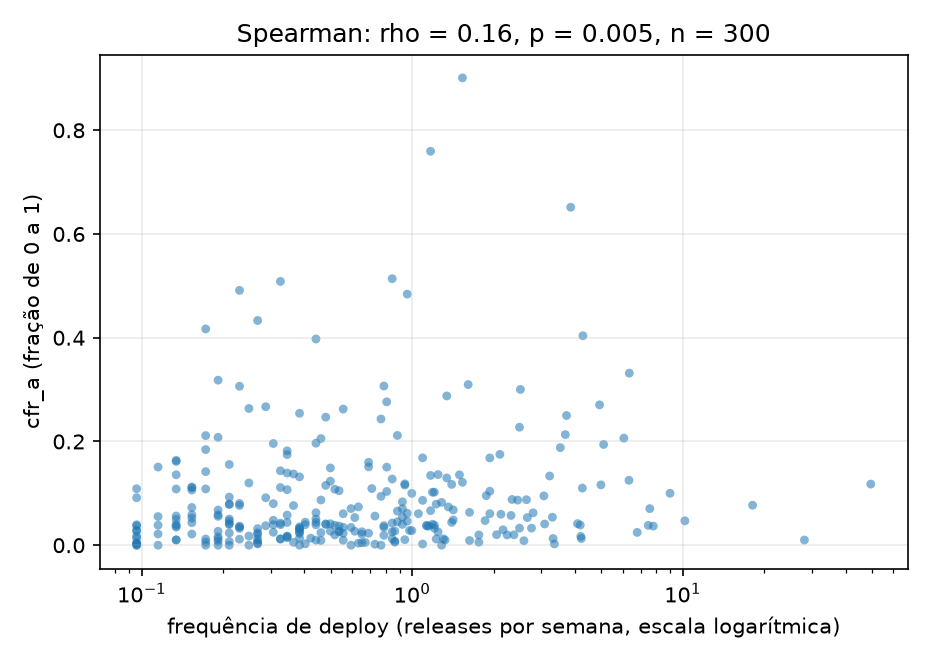
\includegraphics[width=0.48\textwidth]{rq05_cfr_a.png}\hfill
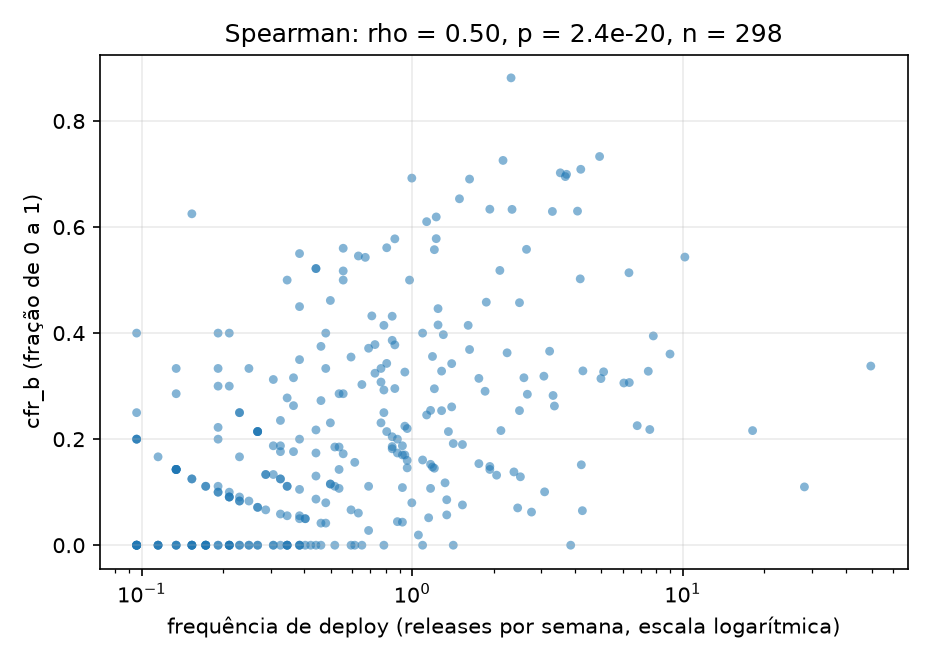
\includegraphics[width=0.48\textwidth]{rq05_cfr_b.png}
\caption{Frequência de deploy (escala logarítmica) e CFR de cada repositório: variante (a), à esquerda, e variante (b), à direita.}
\label{fig:rq05}
\end{figure}

Confirmamos as duas hipóteses. Para o CFR (a), a correlação é fraca ($|\rho| < 0{,}3$), de modo que a frequência de deploy explica pouco da taxa de falha de CI (cerca de 3\% da variação dos postos). O sinal é positivo e significativo, e não nulo: quem publica mais releases tem um pouco mais de execuções com falha. Para o CFR (b), a correlação positiva e moderada que esperávamos ficou no limite entre moderada e forte. As duas variantes levam a conclusões diferentes sobre o \textit{trade-off} entre velocidade e estabilidade: o CFR (a) indica quase independência, em linha com o DORA \cite{dora2024report}, e o CFR (b) indica que mais releases vêm com mais correções. Esse segundo resultado é em parte efeito da definição, pois quem publica mais releases tem mais chance de ter uma correção em até 7 dias, e não deve ser lido como prova de que a velocidade causa instabilidade.

\subsection{RQ 06: características associadas ao desempenho}

Foram feitos 20 testes (cinco fatores e quatro métricas), e só 4 continuam significativos após a correção de Holm, todos com $p < 0{,}001$ (Tabela~\ref{tab:rq06}). A idade tem o maior efeito: os repositórios mais novos publicam mais releases e têm lead time menor. Com mais contribuidores, o lead time também é maior. A linguagem se associa ao lead time com efeito médio. Nenhum fator se associa significativamente ao CFR (a) nem ao tempo de recuperação, e a popularidade (estrelas) e o tipo do projeto não mostram associação significativa com nenhuma métrica ($p$ ajustado de 0,54 a 1,0; o tipo cobre só 58 repositórios, 54 na recuperação).

\begin{table}[ht]
\centering
\small
\caption{Comparações significativas após a correção de Holm (todas com $p < 0{,}001$) e medianas por grupo. Os quartis de idade vão de 110 a 931 dias (Q1) até 3.936 a 6.746 dias (Q4), e os de contribuidores, de 8 a 223 (Q1) até 1.070 a 9.908 (Q4).}
\label{tab:rq06}
\begin{tabular}{llrp{0.32\textwidth}}
\hline
Fator e métrica & $\varepsilon^2$ & n & Mediana por grupo \\
\hline
Idade e lead time (a) & 0,365 (grande) & 299 & Q1 a Q4: 51, 204, 477 e 1.024 h \\
Contribuidores e lead time (a) & 0,183 (médio) & 299 & Q1 a Q4: 131, 179, 220 e 981 h \\
Idade e frequência & 0,118 (médio) & 300 & Q1 a Q4: 0,94, 0,61, 0,35 e 0,36 por semana \\
Linguagem e lead time (a) & 0,095 (médio) & 299 & Python 131 h, TypeScript 217 h e Rust 183 h; Go 567 h e outras 658 h \\
\hline
\end{tabular}
\end{table}

Confirmamos que poucas comparações permanecem significativas (4 de 20), e que a popularidade e o tamanho do efeito da maioria são pequenos. As demais expectativas não se confirmaram. Esperávamos as maiores associações com os contribuidores e o tipo do projeto, mas a maior foi com a idade, que prevíamos pequena, e o tipo do projeto não apresentou nenhuma. Os contribuidores se associam ao lead time, mas no sentido oposto ao esperado: os projetos com mais contribuidores levam mais tempo, e não menos, para publicar o que foi escrito, sem efeito na frequência nem na recuperação. Uma explicação plausível, que não testamos, é que projetos mais antigos e maiores têm processos de release mais cautelosos e mais commits acumulados entre uma release e outra. A análise por fator isolado não separa idade e contribuidores, que podem andar juntos, e o tamanho do efeito da idade (grande) sugere que ela é o fator mais importante da amostra.
